
\documentclass[border={0pt 0pt 0pt 0pt}]{standalone}
\usepackage{tikz-cd,tikz-3dplot} 
\usetikzlibrary{calc,intersections,through,backgrounds,decorations.pathmorphing, decorations.shapes,decorations.markings,patterns,angles}
%include other needed packages here   
\begin{document}
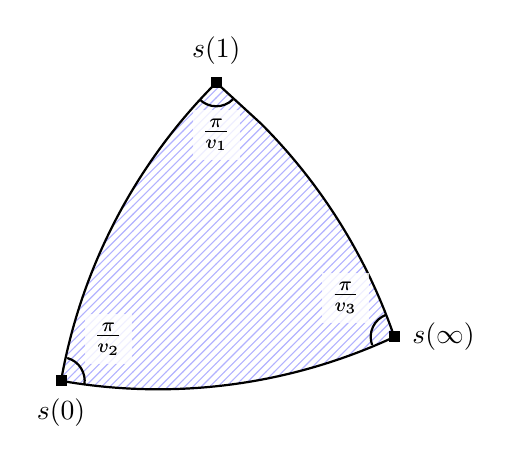
\begin{tikzpicture}[scale=3]
\def\a{2.366025403784439} 
\coordinate (A) at (0,0);
\draw[thick,pattern=north east lines, pattern color=blue!30!white](A) arc [start angle=135, end angle=170, radius=\a] coordinate(B)arc [start angle=-100, end angle=-65, radius=\a]coordinate(C) arc [start angle=19, end angle=45, radius=\a] --cycle;

\foreach \point/\angla/\anglb/\lab/\position in {A/-135/-45/1/below, B/75/-10/2/above right, C/200/110/3/above left}
{
	\draw[thick] ($(\point)+(\angla:1mm)$) arc [start angle=\angla, end angle=\anglb, radius=1mm]  node[midway,\position=1pt,fill=white,fill opacity=0.8]{$\frac{\pi}{v_\lab}$} node[midway,\position=1pt]
{$\frac{\pi}{v_\lab}$};
}
\foreach \point/\position/\lab in {A/above/s(1),B/below/s(0),C/right/s(\infty)}
{
	\node [fill=black,inner sep=2pt]  at (\point){};
	\node[\position=3pt] at (\point) {$\lab$};
}
\end{tikzpicture}
\end{document}